\documentclass{tufte-book}
\usepackage[utf8]{inputenc}
\usepackage[english]{babel}
\usepackage{amsmath,amsthm,amssymb}
\usepackage{eso-pic}
\usepackage{tikz}
\usepackage{multicol}
\usepackage{graphicx}
\graphicspath{{../images/}}

% cover photo
\newcommand\BackgroundPic{%
\put(0,-220){%
\parbox[b][\paperheight]{\paperwidth}{%
\vfill
\centering
\includegraphics[height=1.3\paperheight,%
keepaspectratio]{chemcover2}%
\vfill
}}}

\setlength{\parindent}{0pt}
\renewcommand{\emph}[1]{\textbf{#1}}

\title[Chemistry \& Materials Science]{%
  \setlength{\parindent}{0pt}%
Chemistry \& \par Materials \par Science}
\author{Richard Robinson}
\begin{document}
\AddToShipoutPicture*{\BackgroundPic}
\frontmatter
\maketitle
\setlength{\parindent}{0pt}
\mainmatter

% ------------------------------------------------------------------- %
% MAIN DOCUMENT
% ------------------------------------------------------------------- %

\chapter{Introduction}

\section{Stoichiometry}

\textsc{All stoichiometric} equations for quantities may be derived from \begin{equation}
  n_1/v_1 = n_2/v_2
\end{equation}
The \emph{percentage yield} is defined as \begin{equation}
  \text{\% yield} = \frac{\text{actual yield}}{\text{theo. yield}} \times 100 \%
\end{equation}

A crucial aspect in confirming stoichiometric results is using \emph{dimensional analysis}; that is, using the dimensions of each unit in the equation(s) and confirming the final unit has the proper dimensions.
\begin{center}
  \begin{tabular}{ll}
    moles & $n = m/M = CV$ \\
    atoms & $n_{\mathrm{atoms}} = \rho V N_a / M$ \\
    molarity & $C = mn/MV$ \\
    dilution & $n_1 = n_2$
  \end{tabular}
\end{center}

\section{Bonding}

\begin{marginfigure}[3cm]
\begin{center}
  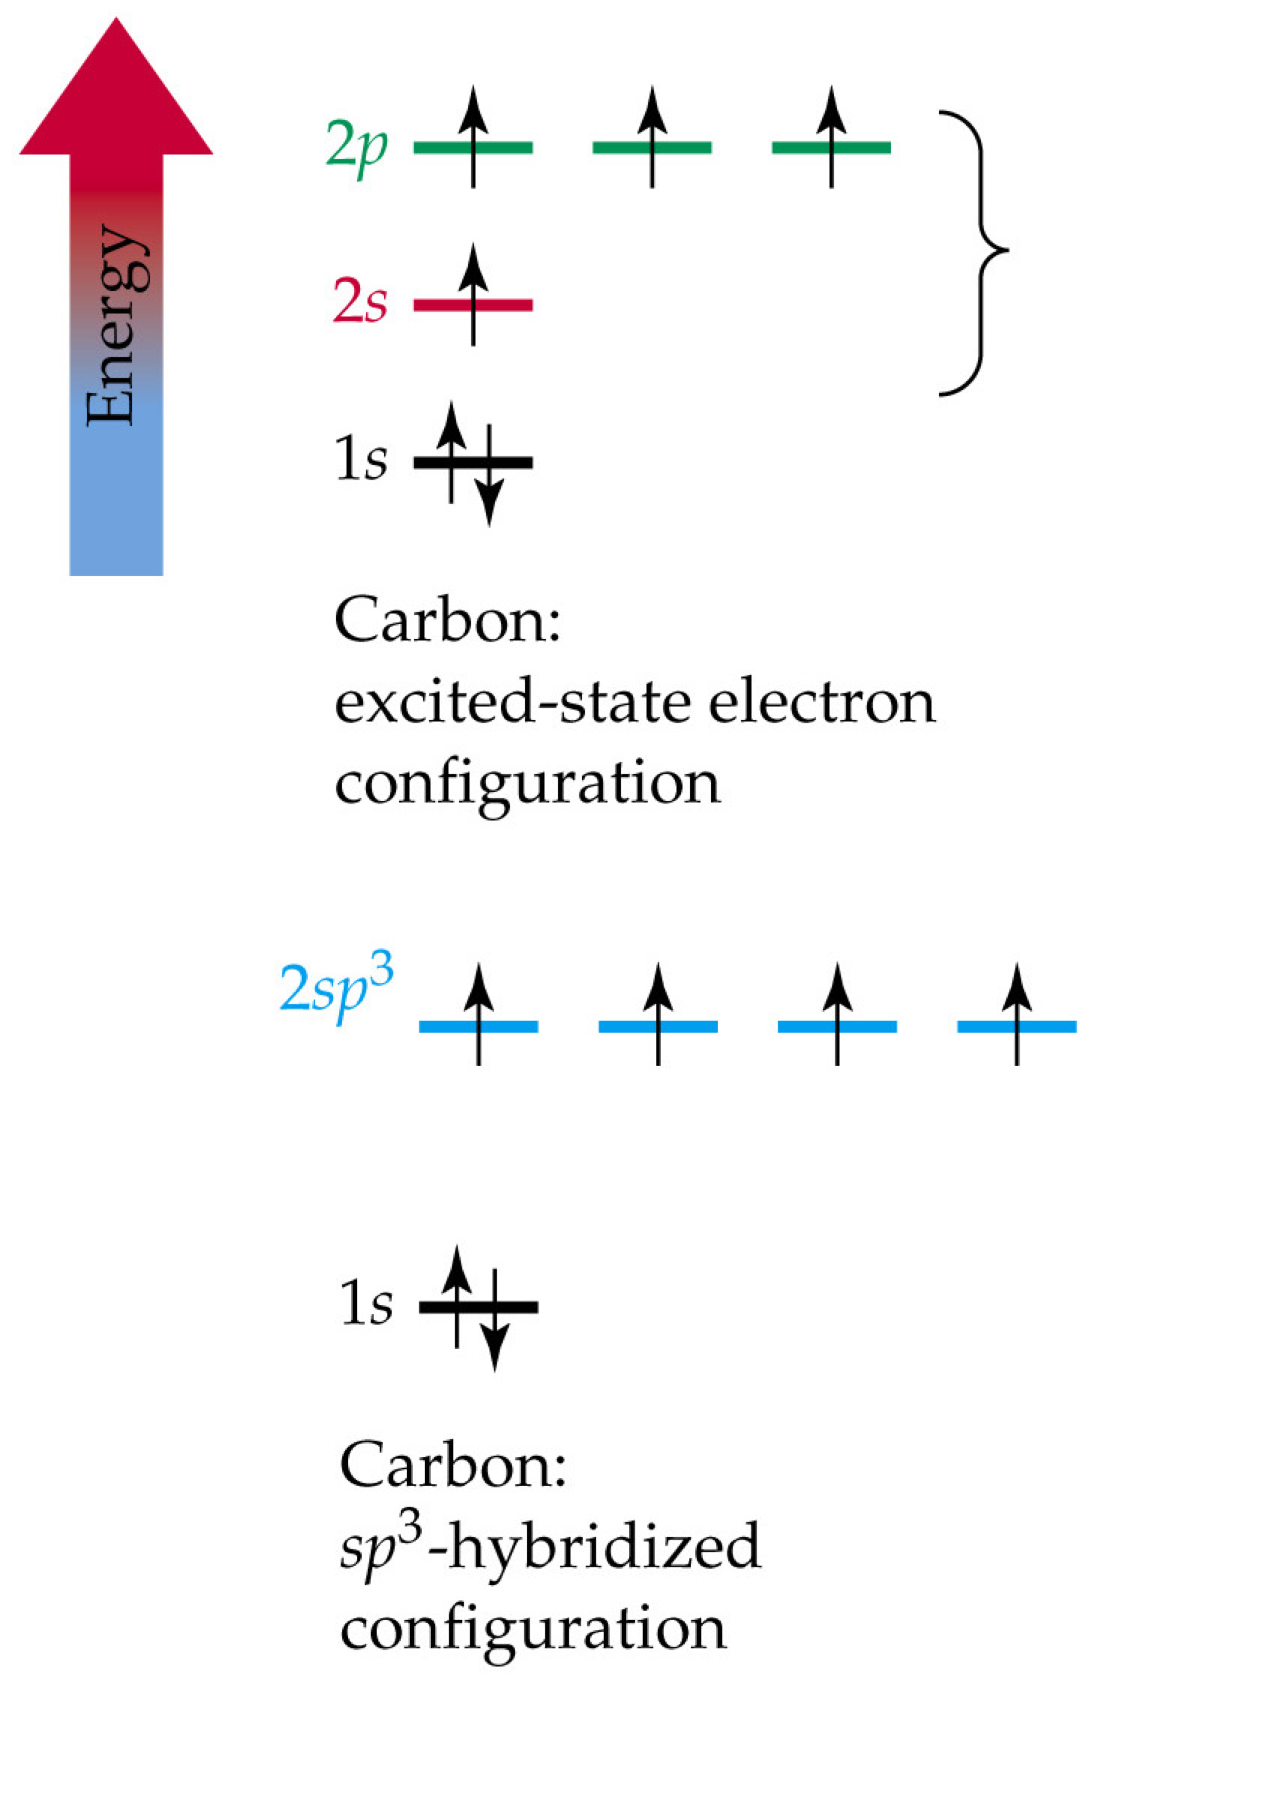
\includegraphics[width=0.9\textwidth]{orbitals} \phantom{mmm}
\end{center}
\end{marginfigure}
%
The total number of \emph{orbitals} is equal to $n^2$, where $n$ is the principle quantum number, wherein each orbital has a maximum of two electrons. The orbitals are filled in the order of \begin{equation}
  1s^2 \, 2s^2 \, 2p^6 \, 3s^2 \, 3p^6 \, 4s^2 \, 3d^{10} \, 4p^6 \, 5s^2 \dots
\end{equation}
This maximum occurs only if all subshells contain one electron originally, known as Hund's rule.

\begin{center}
  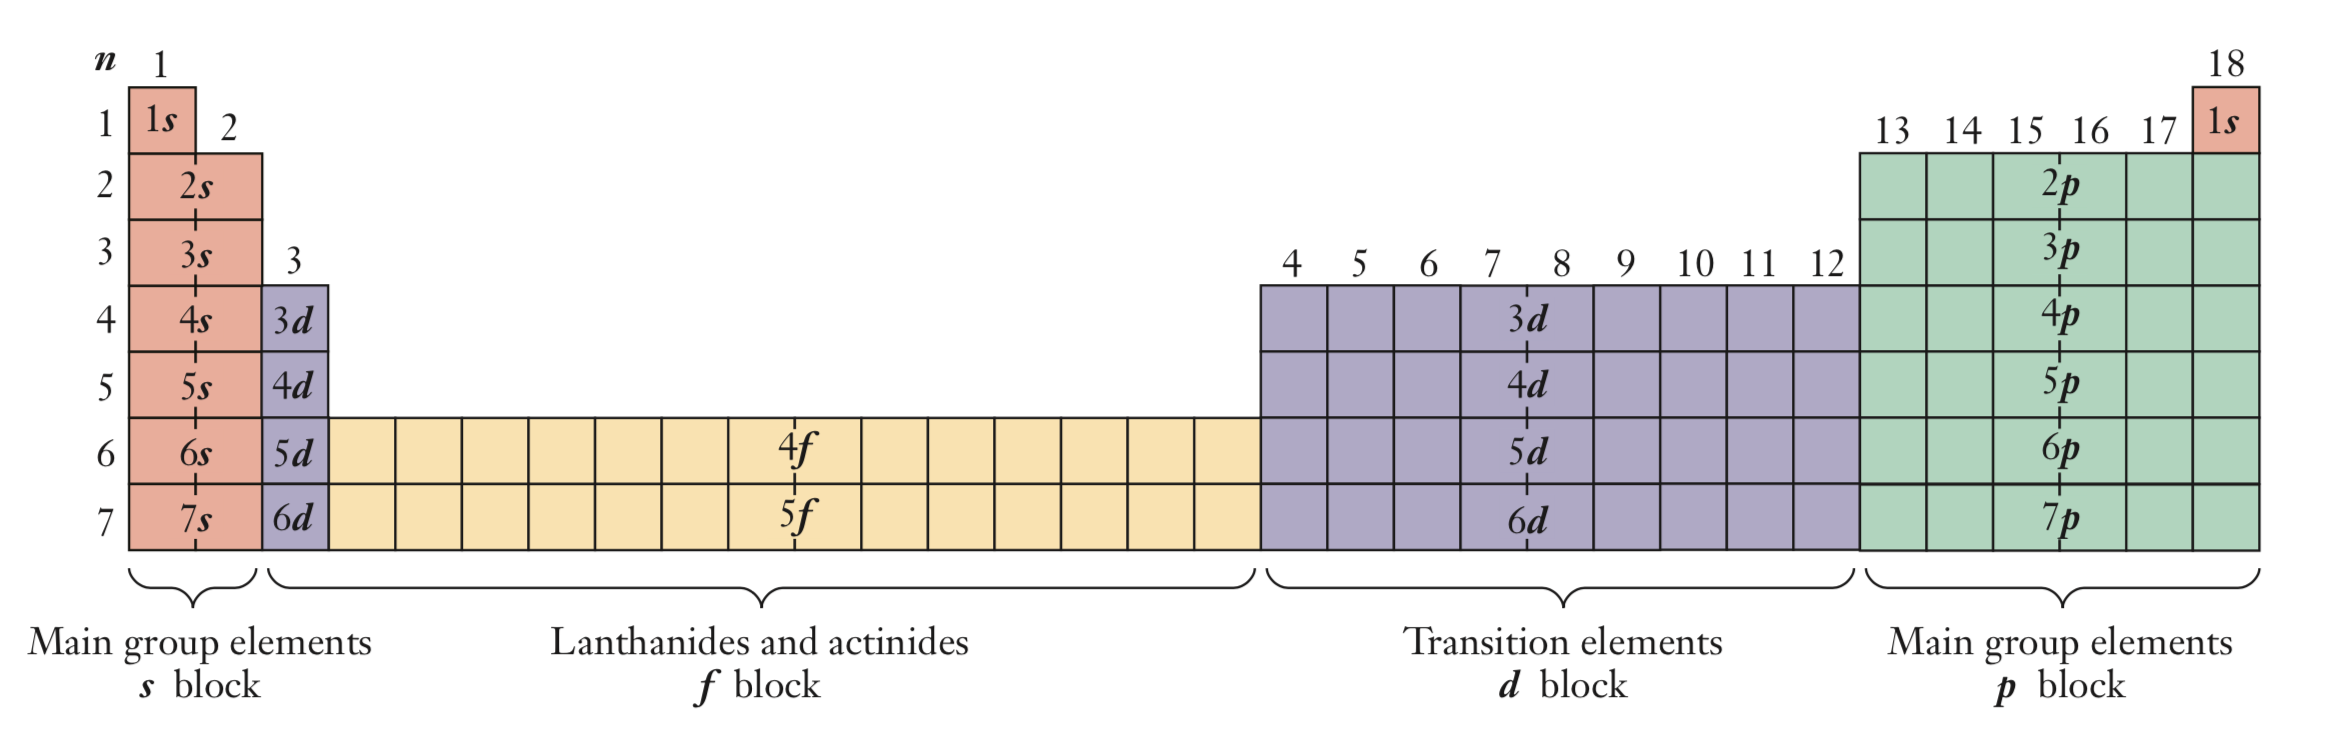
\includegraphics[width=\textwidth]{table}
\end{center}

The \emph{formal charge} is given by $q_f = n_v - n_l - \frac{1}{2} n_s$ in which $\sum q_f = 0$, where $n_v$ is the total number of valence electrons; $n_l$ is the number of lone pairs; and $n_s$ is the number of electrons shared in bonds.
%
\begin{marginfigure}
\begin{center}
  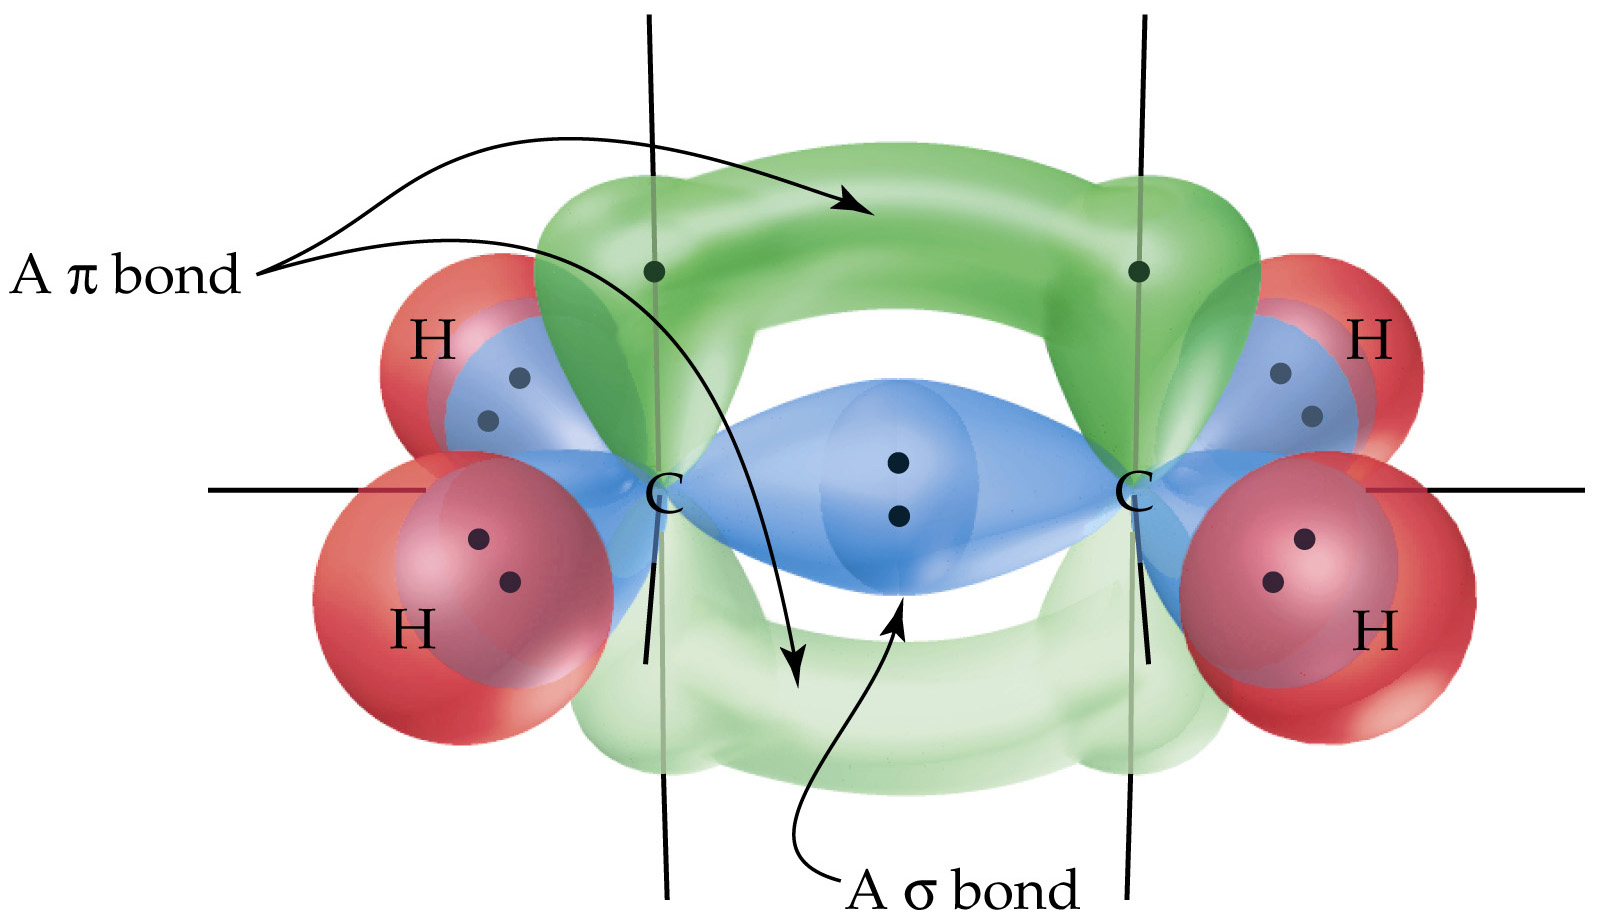
\includegraphics[width=0.78\textwidth]{bonds} \phantom{mmmm}
\end{center}
\end{marginfigure}
\marginnote[2mm]{Sigma and pi bonds overlapping for hybridization.}
%
\bigskip
\emph{Hybrid orbitals} are dependent on molecular geometry, and filled by $sp^3d^2$. The number of orbitals is equal to the number of electron pairs. The number of \emph{sigma and pi bonds} is equal to \begin{equation}
  n_\sigma = \sum n_\text{all} \quad\text{and}\quad n_\pi = \sum n_\text{dbl} + 2 \sum n_\text{tri}
\end{equation}
Other properties of the periodic table include \begin{itemize}
  \item Atomic size increases toward the bottom left;
  \item Ionization energy and electronegativity increase towards the top right;
\end{itemize}

\section{Atoms \& Molecules}
\begin{marginfigure}[3cm]
\begin{center}
  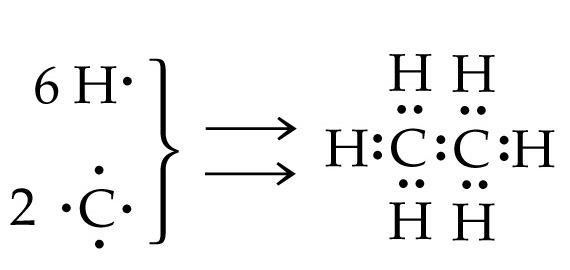
\includegraphics[width=0.7\textwidth]{lewis} \phantom{mmmm}
\end{center}
\end{marginfigure}
\marginnote[1mm]{Constructing a lewis dot structure.}
\emph{Lewis dot structures} are created via the following algorithm: \begin{enumerate}
  \item Count the total number of valence electrons in the molecule
  \item Place single bonds between all connected atoms;
  \item Place the remaining valence electrons not accounted for in (2) on individual atoms, specifically as lone pairs whenever possible;
  \item Create multiple bonds as needed for any atoms that do not have a full octet
\end{enumerate}

% ------------------------------------------------------------------- %
% EQUILIBRIUM
% ------------------------------------------------------------------- %

\chapter{Chemical Equilibrium}

\section{Equilibrium Constants}

A system is said to be at \emph{dynamic equilibrium} if the rates of both reactions are equal but do not approach zero. For a general chemical reaction, the reaction quotient and equilibrium constant are
%
\begin{marginfigure}[5mm]
\begin{center}
  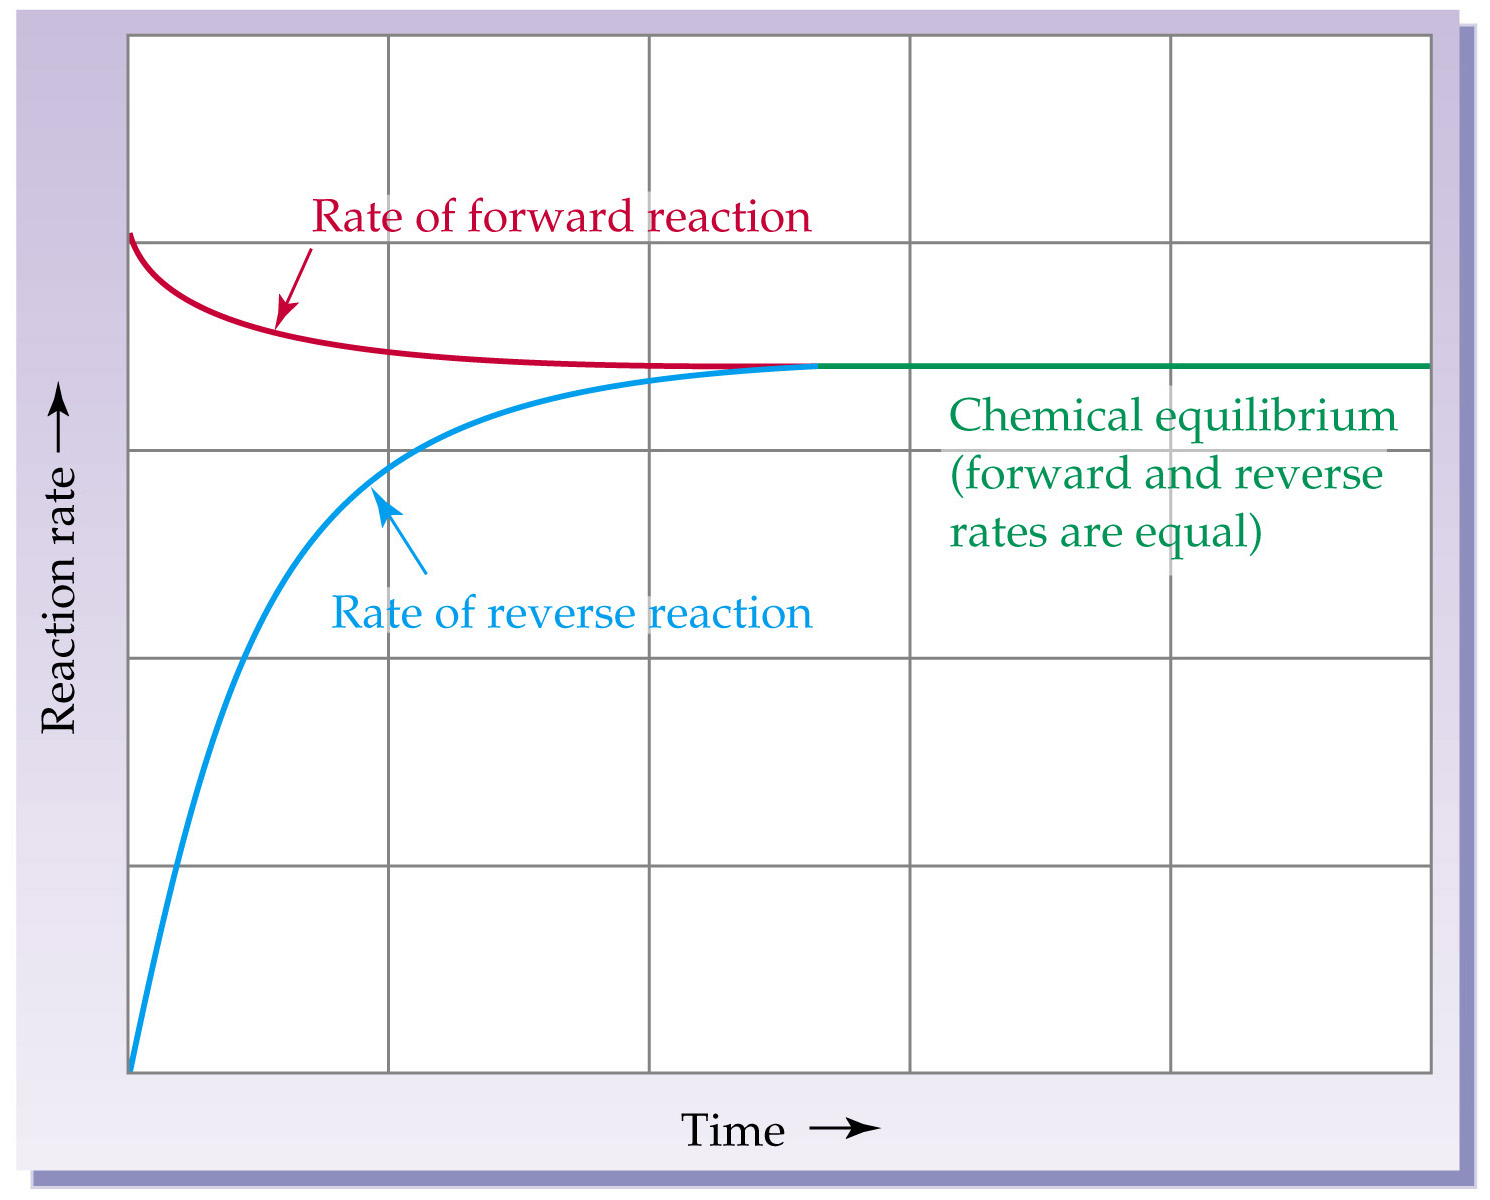
\includegraphics[width=0.9\textwidth]{equilibrium} \phantom{m}
\end{center}
\end{marginfigure}
\marginnote[2mm]{Dynamic equilibrium.}
%
\begin{equation}
  Q = \frac{[C]^c [D]^d}{[A]^a [B]^b} \quad\text{and}\quad K_c = \frac{[C]^c_{eq} [D]^d_{eq}}{[A]^a_{eq} [B]^b_{eq}}
\end{equation}
respectively. For reactions which take place in the gas phase, \begin{equation}
  K_p = K_c RT^{\Delta n_g} \iff [X] \equiv P_X = [X]RT
\end{equation}
where $\Delta n_g = c+d-(a+b)$. Reactions are \emph{homogeneous} iff all constituents are either exclusively gaseous or aqueous. Incidentally, in a heterogeneous reaction, $K$ only includes the compounds in the reaction which are not solid nor liquid. For a series of reactions, \begin{equation}
  K_n = \prod K_i
\end{equation}
The procedure to calculate \emph{final concentrations} of specific compounds in a reaction $A \leftrightharpoons B$ is as follows:
\begin{enumerate}
  \item For reactants and products, $[A_i]_{eq} = [A_i] \mp ax$, respectively.
  \item Using these concentrations in $K$, solve for $x$.
  \item Substitute $x$ into the original equilibrium concentrations.
\end{enumerate}
\begin{center}
  \begin{tabular}{clll}
    R & $A$ & $A'$ & $B$ \\
    \hline
    I & $[A_i]$ & $[A'_i]$ & $[B_i]$ \\
    C & $-ax$ & $-a'x$ &  $+bx$ \\
    E & $[A]_{eq}$ & $[A']_{eq}$ & $[B]_{eq}$
  \end{tabular}
\end{center}

\section{LeChatelier's Principle}

\emph{LeChatelier's principle} states that when a system at equilibrium is stressed, it reestablishes itself to avoid such stress; that is,
\begin{itemize}
  \item If the concentration of products is increased or reactants decreased, $Q>K$ and more reactants are formed;
  \item If vice versa, $Q<K$ and more products are formed.
\end{itemize}
%
\begin{marginfigure}[5mm]
\begin{center}
  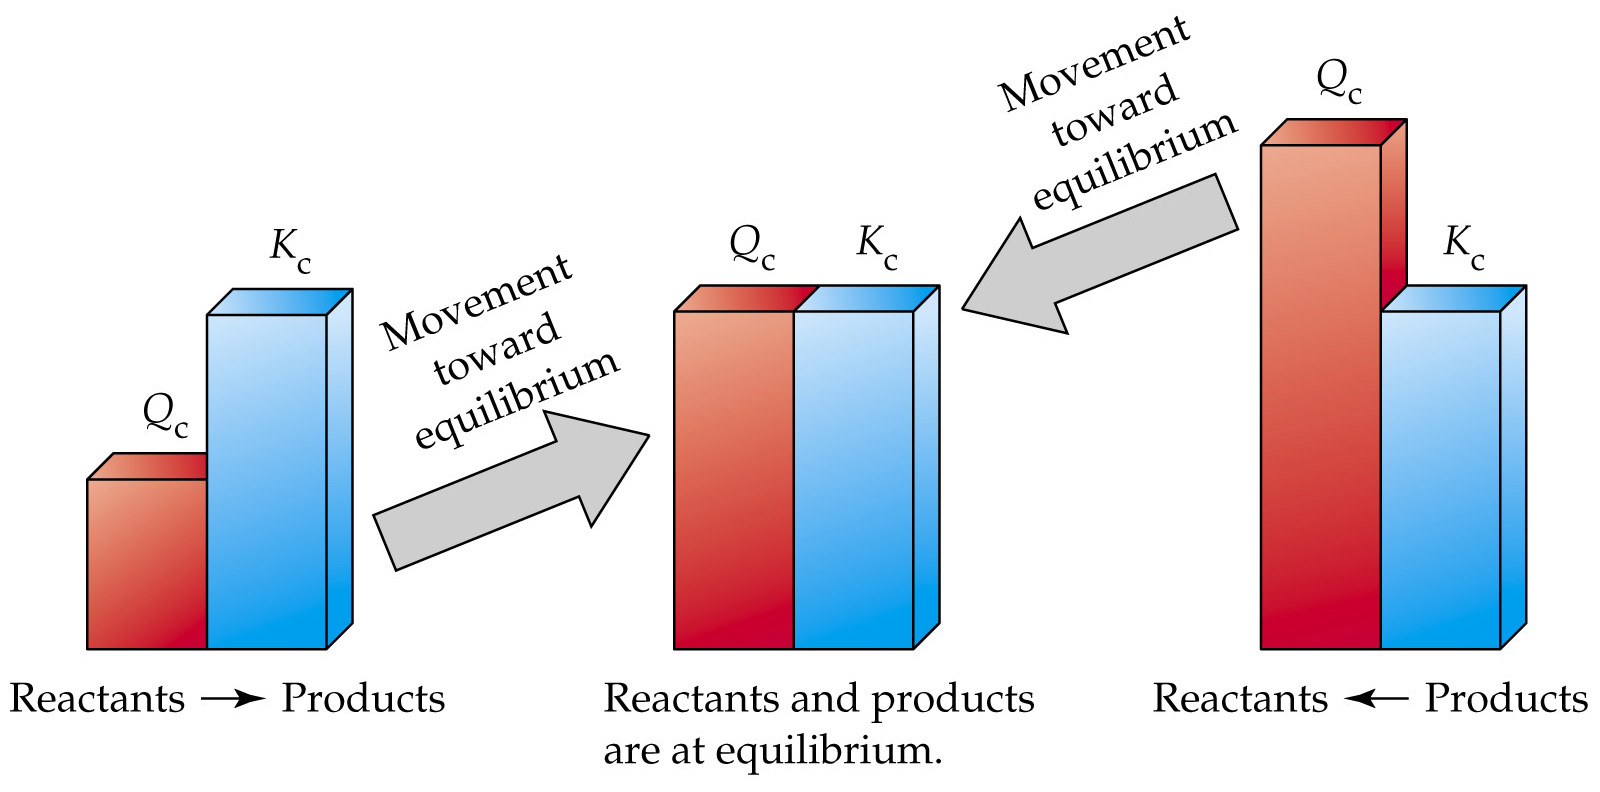
\includegraphics[width=\textwidth]{qk}
\end{center}
\end{marginfigure}
\marginnote[2mm]{Predicting the direction of reaction. The direction of reaction depends on the relative values of $Q$ and $K_c$.}
%
Pressure is inversely proportional to the amount of moles the side to which equilibrium moves to has. Note that catalysts have no effect upon the properties of equilibrium systems, unlike temperature.

\bigskip
\emph{Exothermic reactions} produce heat and endothermic reactions absorb heat. If a reaction is exothermic and temperature increases or vice versa, more reactants are formed. Otherwise, more products are formed.

\section{Solubility Equilibria}
For a reaction $A(s) \leftrightharpoons cC(aq) + dD(aq)$, the solubility constant is defined as \begin{equation}
  K_{sp} = [C]^c [D]^d
\end{equation}
and the molar solubility is \begin{equation}
  x = (K_{sp}/c^cd^d)^{1/(c+d)}
\end{equation}
%
\begin{marginfigure}[5mm]
\begin{center}
  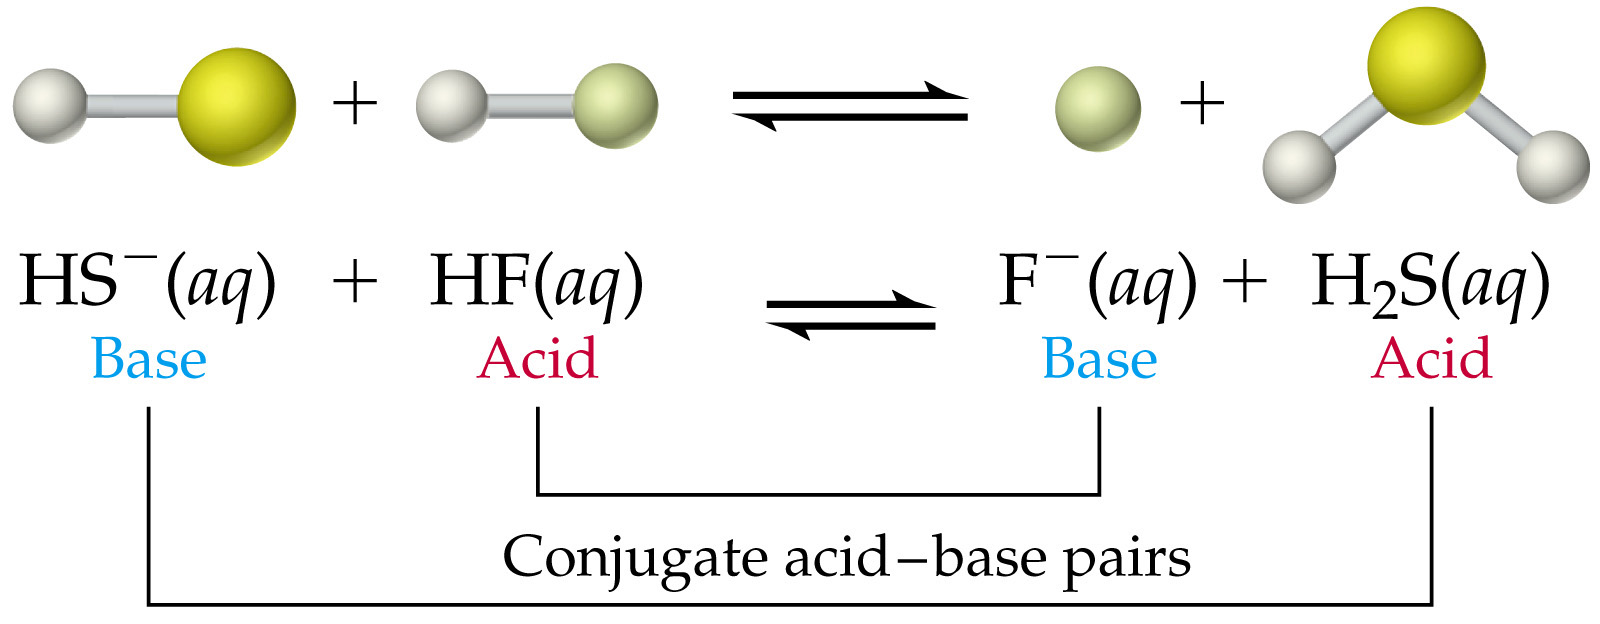
\includegraphics[width=\textwidth]{acidbase}
\end{center}
\end{marginfigure}
\marginnote[2mm]{Conjugate acid-base pairs for the reaction between HS$^-$ and HF.}
%
A Brønsted-Lowry acid is a proton $H^+$ donor, and a base a proton acceptor. The equation for the \emph{dissociation} of a weak acid $HA$ is \begin{equation}
  HA(aq) + H_2O (\ell) \leftrightharpoons H_3O^+ (aq) + A^- (aq)
\end{equation}
snd for a weak base $B$,
\begin{equation}
  B(aq) + H_2O (\ell) \leftrightharpoons BH^+ (aq) + OH^-(aq)
\end{equation}
The acid and base ionization constants are $K_a,K_b = K_s$ respectively such that $[X]_{eq} = [X]_i$ for $X = HA, B$. The \emph{Gibbs free energy} is related to $K$ by \begin{equation}
\Delta G^\ominus = -RT \ln K = H-TS
\end{equation}

% ------------------------------------------------------------------- %
% THERMODYNAMICS
% ------------------------------------------------------------------- %

\chapter{Thermodynamics}

\section{The Second Law}
\textsc{A spontaneous reaction} occurs without the need for continuous intervention. When heating a system, its \emph{entropy} $S$ increases. The second law states that for a spontaneous reaction,
%
\begin{marginfigure}[5mm]
\begin{center}
  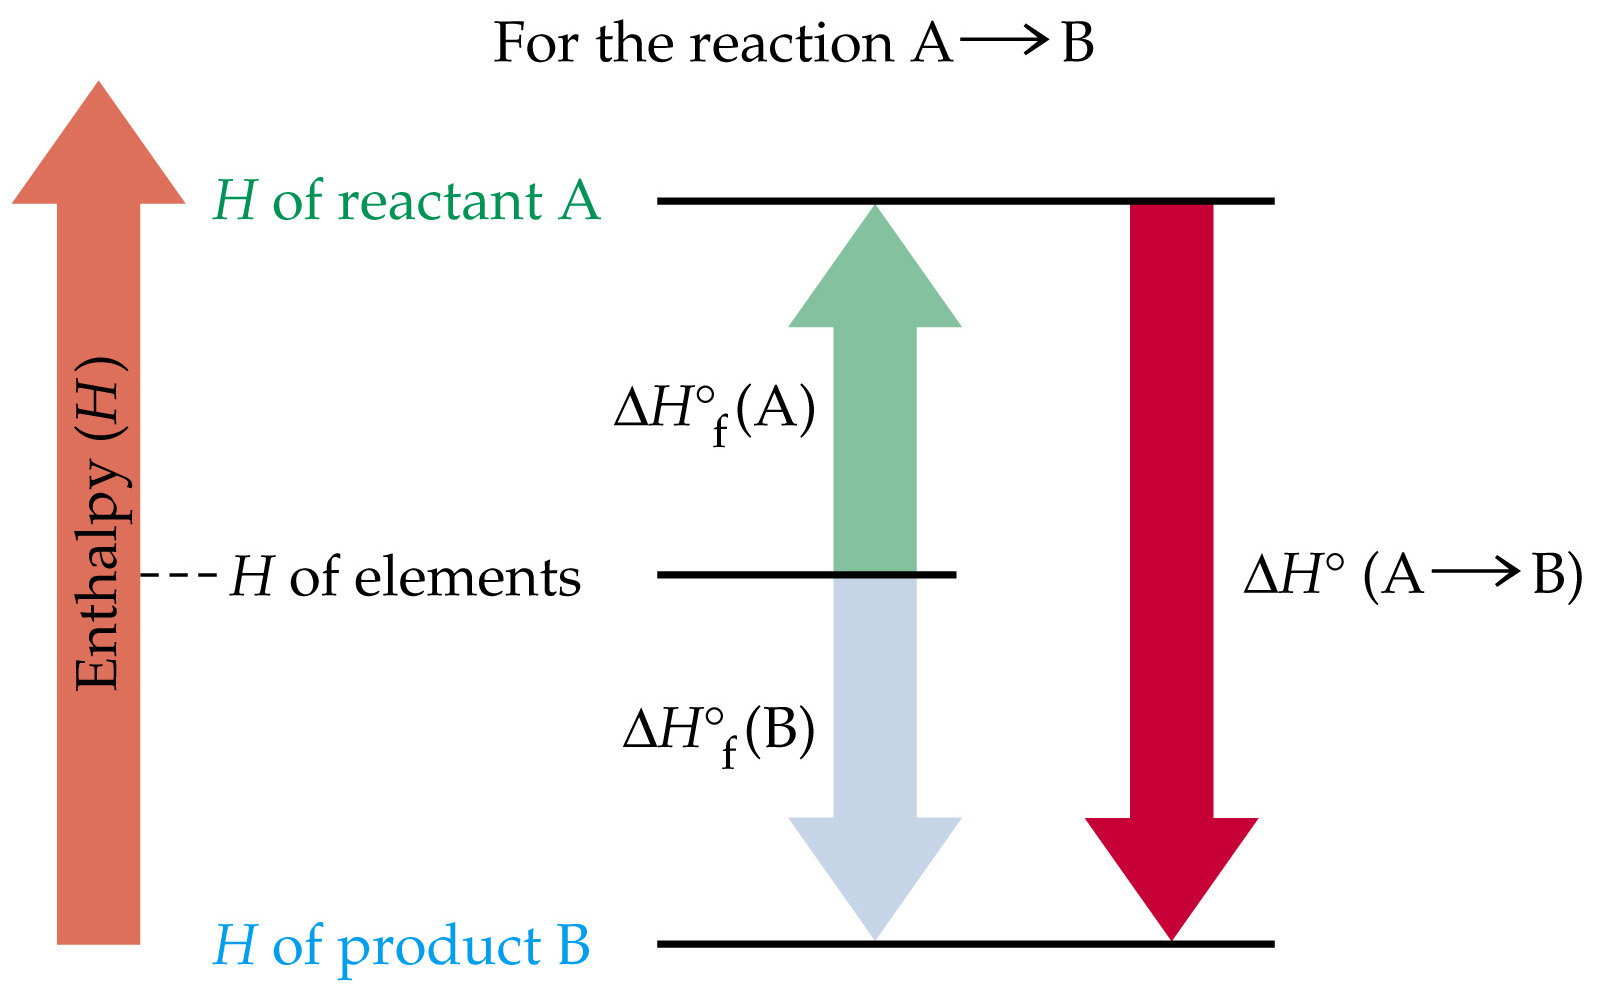
\includegraphics[width=\textwidth]{enthalpy}
\end{center}
\end{marginfigure}
\marginnote[2mm]{The enthalpy $\Delta H^\ominus$ for the  reaction $A\to B$ is the difference between the standard heats of formation of products and reactants.}
%
\begin{equation}
  \Delta S_u = \Delta S + \Delta S_{sur} > 0
\end{equation}
where $\Delta S_{sur} = - \Delta H/T$. If $\Delta \sum v > 0$, then $\Delta S > 0$. The change in standard entropy is \begin{equation}
  \Delta S^\ominus = \Delta \sum v_i S^\ominus_i
\end{equation}
The change in Gibbs free energy is thus also equal to \begin{equation}
  \Delta G = \Delta H - T \Delta S = -T \Delta S_u
\end{equation}
If $\Delta G < 0$, a reaction is spontaneous and vice versa. The change in standard free energy is \begin{equation}
  \Delta G^\ominus = \Delta \sum v_i G^\ominus_i
\end{equation}
Entropy is proportional to $T, r, V, n$ and inversely proportional to $P$.

\section{Enthalpy}

Heat is expressed as $\Delta E - w$. The specific \& molar \emph{heat capacities} are defined as \begin{equation}
  q_s = mc \Delta T \quad\text{and}\quad q_m = nC_p \Delta T
\end{equation}
%
\begin{marginfigure}[-10mm]
\begin{center}
  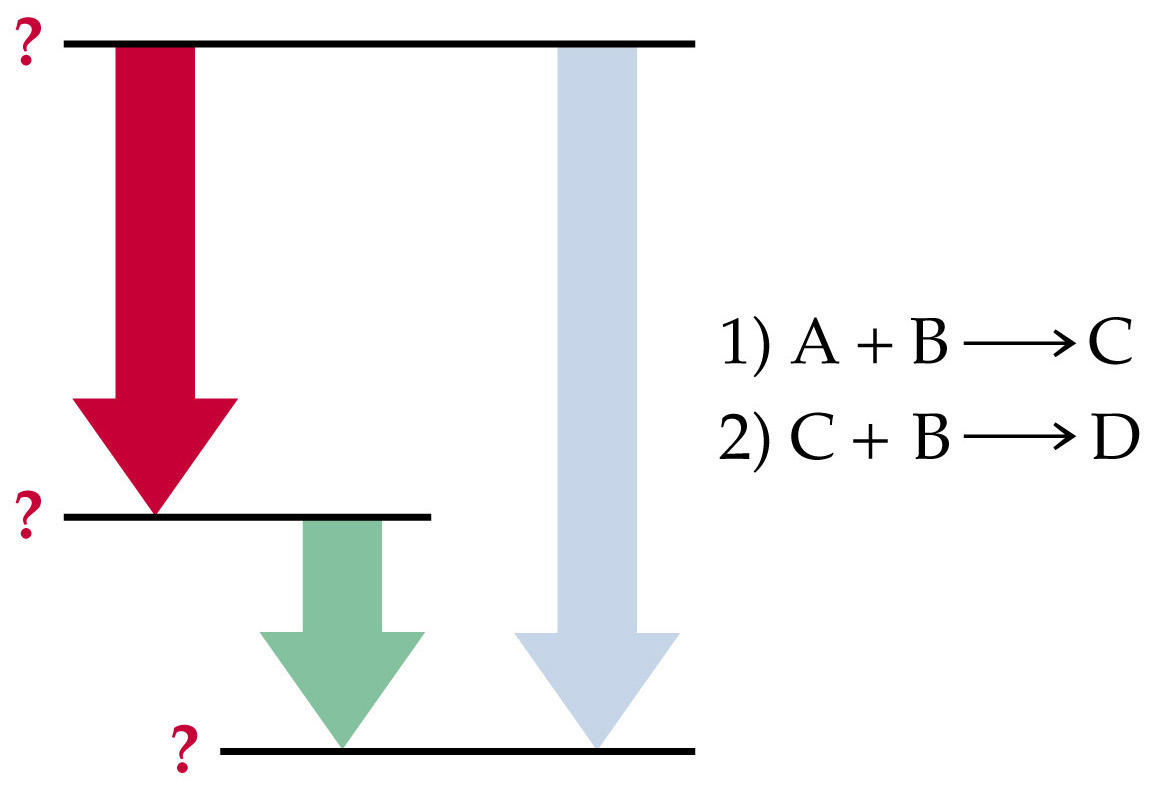
\includegraphics[width=0.9\textwidth]{hess}
\end{center}
\end{marginfigure}
\marginnote[2mm]{Diagram of Hess' Law.}
%
For \emph{calorimetry}, heat is given by \begin{equation}
  q_c = -(q / \Delta T_i) \Delta T_f
\end{equation}
\emph{Enthalpy} is defined as \begin{equation}
  \Delta H = \Delta E + \Delta (PV) = q_p - n \Delta H_{\Delta \text{phase}}
\end{equation}
A reaction is exothermic for $\Delta H<0$ and vice versa. A \emph{formation reaction} is one in which one mole of a compound is formed from its elements such that
\begin{equation}
  aA + bB = 1AB \qquad \Delta H^\ominus = \Delta H_f^\ominus [AB]
\end{equation}
\emph{Hess's Law} states the enthalpy change of a process is independent of path; that is, $\Delta H = \sum \Delta H_i$ meaning that sub-reactions and their enthalpies may be summed together to yield the desired reaction and its enthalpy. The change in standard enthalpy is \begin{equation}
  \Delta H^\ominus = \Delta \sum v \Delta H_f^\ominus
\end{equation}
In thermodynamical equations, always convert to moles from mass or molarity using \begin{equation}
  q = \pm n \Delta H / N_a
\end{equation}
%
\begin{marginfigure}[-50mm]
\begin{center}
  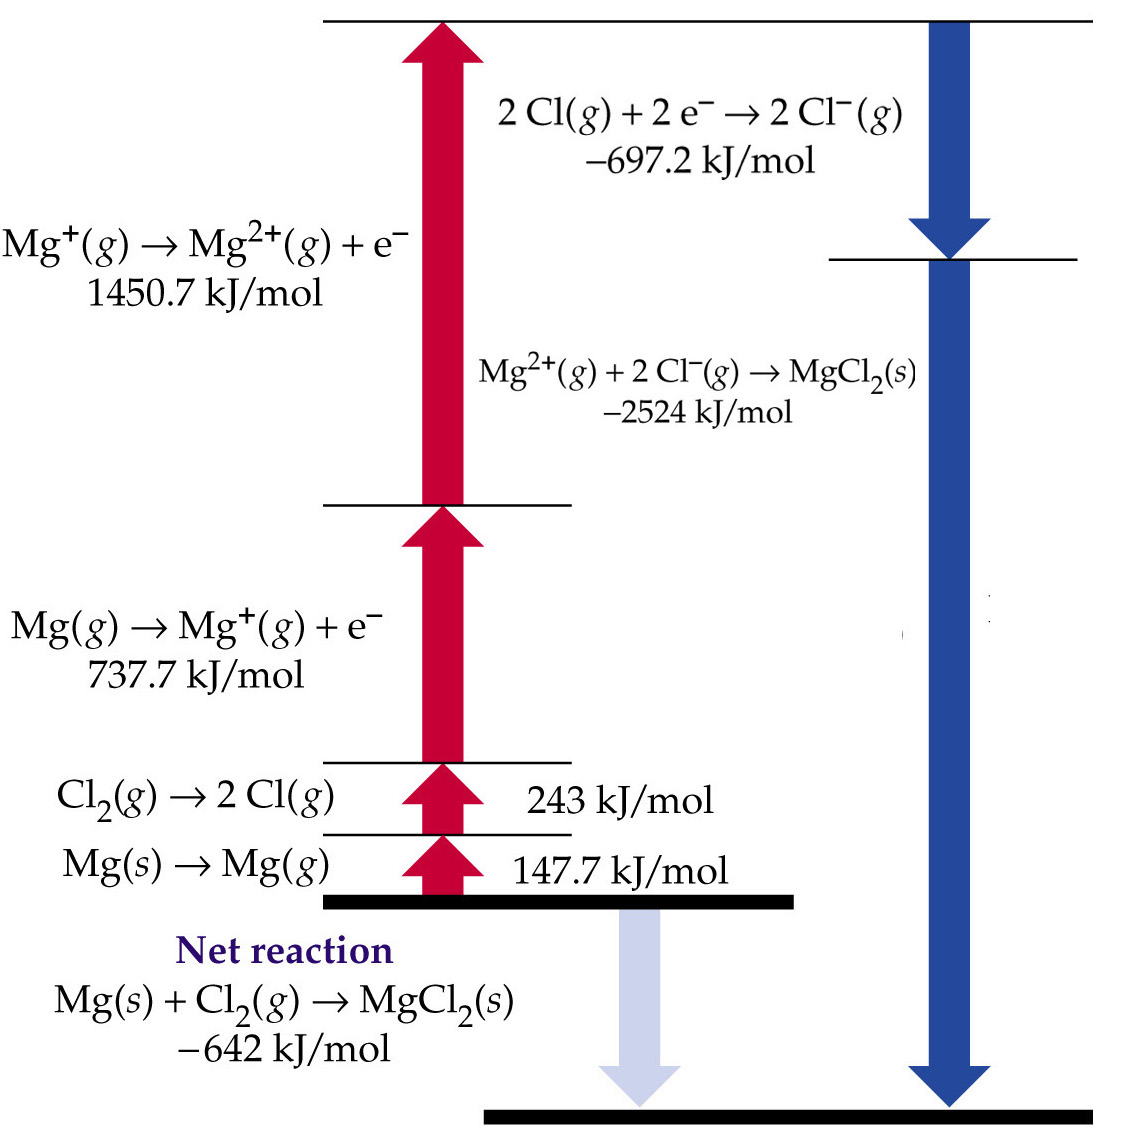
\includegraphics[width=\textwidth]{bornhaber}
\end{center}
\end{marginfigure}
\marginnote[2mm]{Using the Born-Haber cycle to calculate the enthalpy of formation.}
%
The \emph{Born-Haber cycle} is used to find the $H_f$ of an ionic compound $MX$, given by \begin{equation}
  \Delta H_f = H_{\text{sub}} + \textstyle{\frac{1}{2}} B_X + IE_M - EA_X + LE
\end{equation}
where $B$ is the bond energy of $X_2$ from $M + \frac{1}{2} X_2 \to MX$, and LE is defined as exothermic.

% ------------------------------------------------------------------- %
% MATERIALS SCIENCE
% ------------------------------------------------------------------- %

\chapter{Materials Science}

\section{Crystal Structures}
\textsc{Maximum packing} density is achieved with ccp and hcp configurations. The cubic unit cell may be one of sc, bcc, or fcc. The number of atoms per unit cell is equal to $1 \over 2$ number of face--centered atoms + $1 \over 8$ number of atoms.
\begin{center}
  \begin{tabular}{llll}
    & $n$ & cn & a$_0$ \\
    \hline
    sc & 1 & 6 & $2r$ \\
    bcc & 2 & 8 & $4r / \sqrt 3$ \\
    fcc & 4 & 12 & $2 \sqrt 2r$
  \end{tabular}
\end{center}
%
\begin{marginfigure}[-10mm]
\begin{center}
  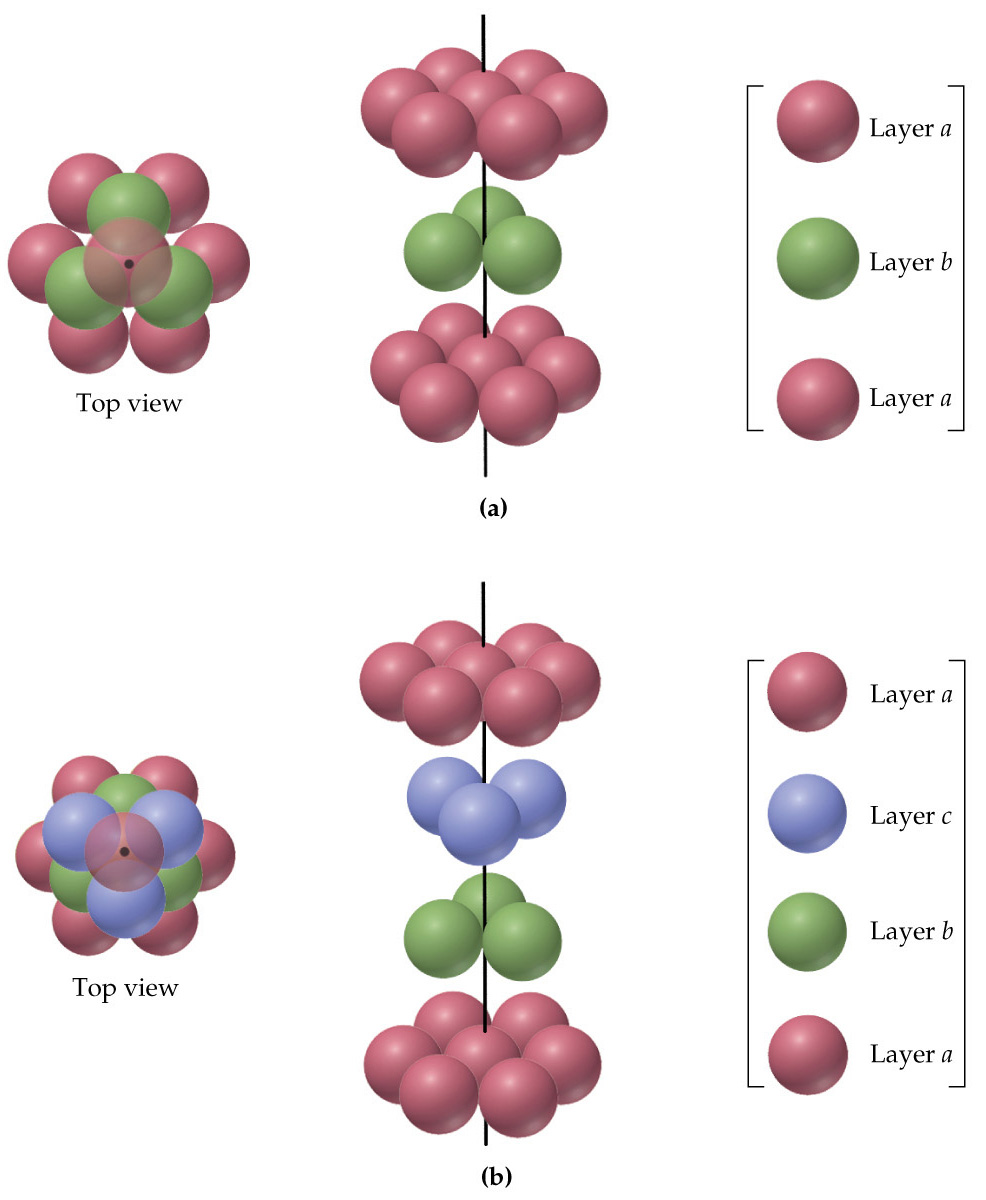
\includegraphics[width=0.8\textwidth]{matsci}
\end{center}
\end{marginfigure}
\marginnote[2mm]{(a) hexagonal close packing and (b) cubic close packing.}
%
The density of a cell is given by \begin{equation}
  \rho = \frac{m}{a^3} \quad\text{for}\quad m = \frac{nM}{N_a}
\end{equation}
The \emph{packing efficiency} of a lattice is defined as $n V_{\text{sph}} / a^3$.

\section{Types of Bonding}
The concept of \emph{band theory} describes metallic bonding in \emph{semiconductors}. In metals / conductors, semiconductors, and insulators, the gap between the lower valence and upper conduction bands is negligible, moderate, and large, respectively.

\bigskip
In an \emph{n-type s}emiconductor, donor electrons are promoted easily into the conduction band, and the dopant has more valence electrons than the semiconductor. Likewise, in a p-type, vice versa. In semiconductors, temperature is proportional to conductivity, and opposite for conductors.

\begin{marginfigure}
\begin{center}
  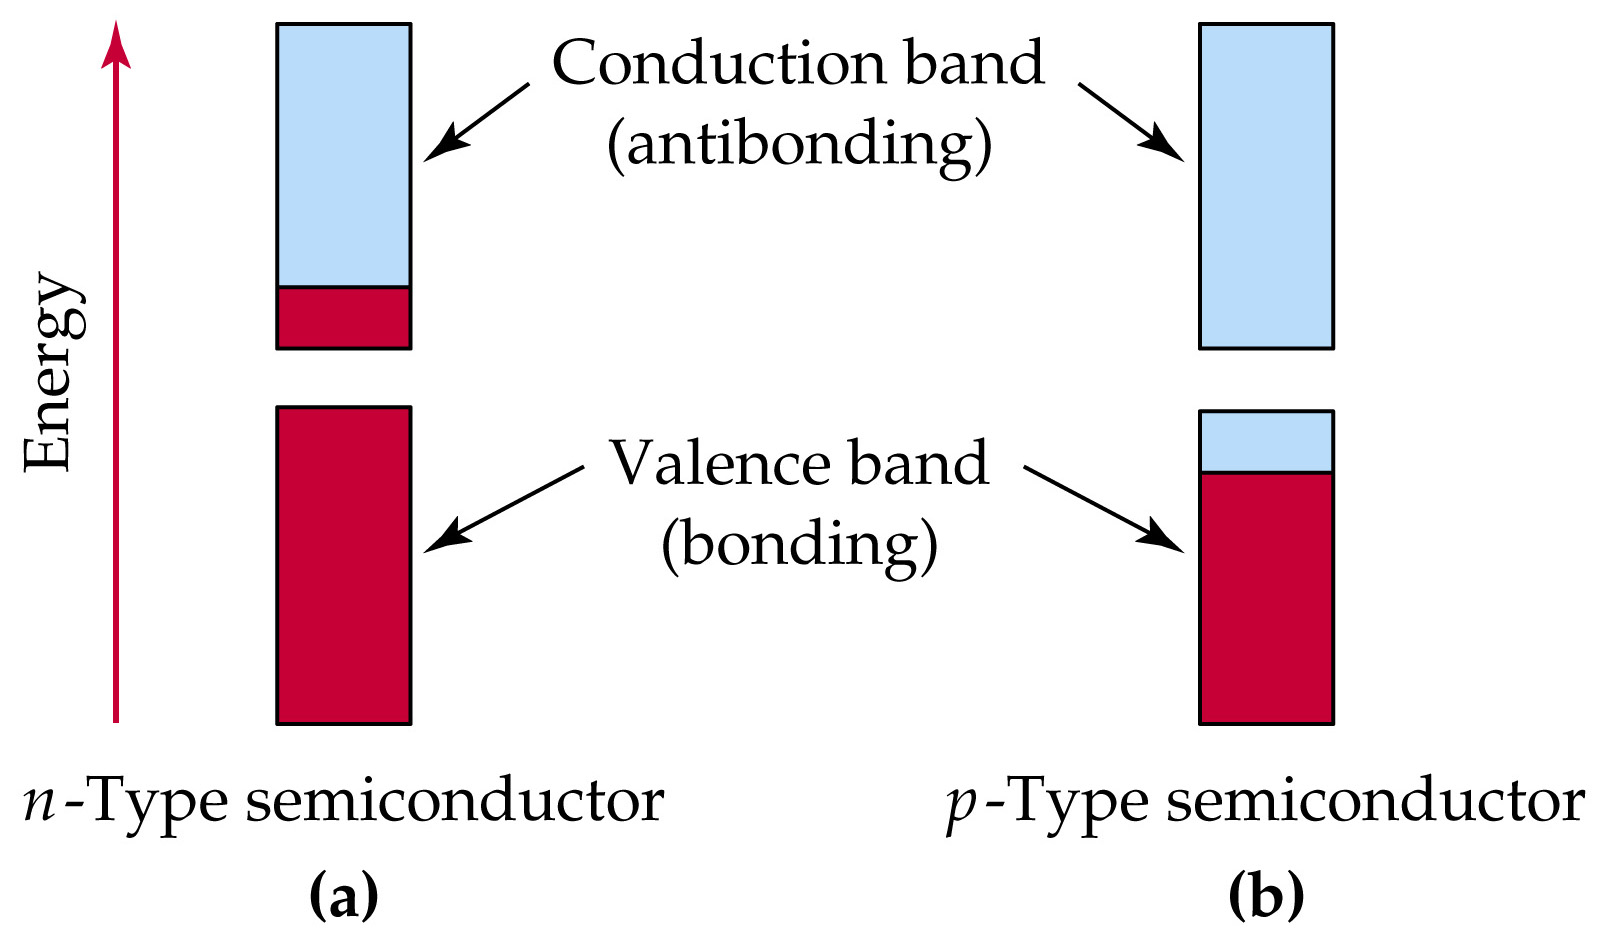
\includegraphics[width=\textwidth]{semi}
\end{center}
\end{marginfigure}
\marginnote[1mm]{The band theory for semiconductors.}

\bigskip
\emph{Hydrogen bonding} is the strongest intermolecular force, and occurs between a hydrogen atom and a highly electronegative atom. \emph{Dipole force} occur for non-symmetrical compounds, and \emph{dispersion forces} occur in the absence of the former three.

\section{Condensed Phases}
In the liquid state, the force is proportional to boiling point, viscosity, number of OH$^-$ ions, $H$, and inversely proportional to vapor pressure and $T$.
%
\begin{marginfigure}[0mm]
\begin{center}
  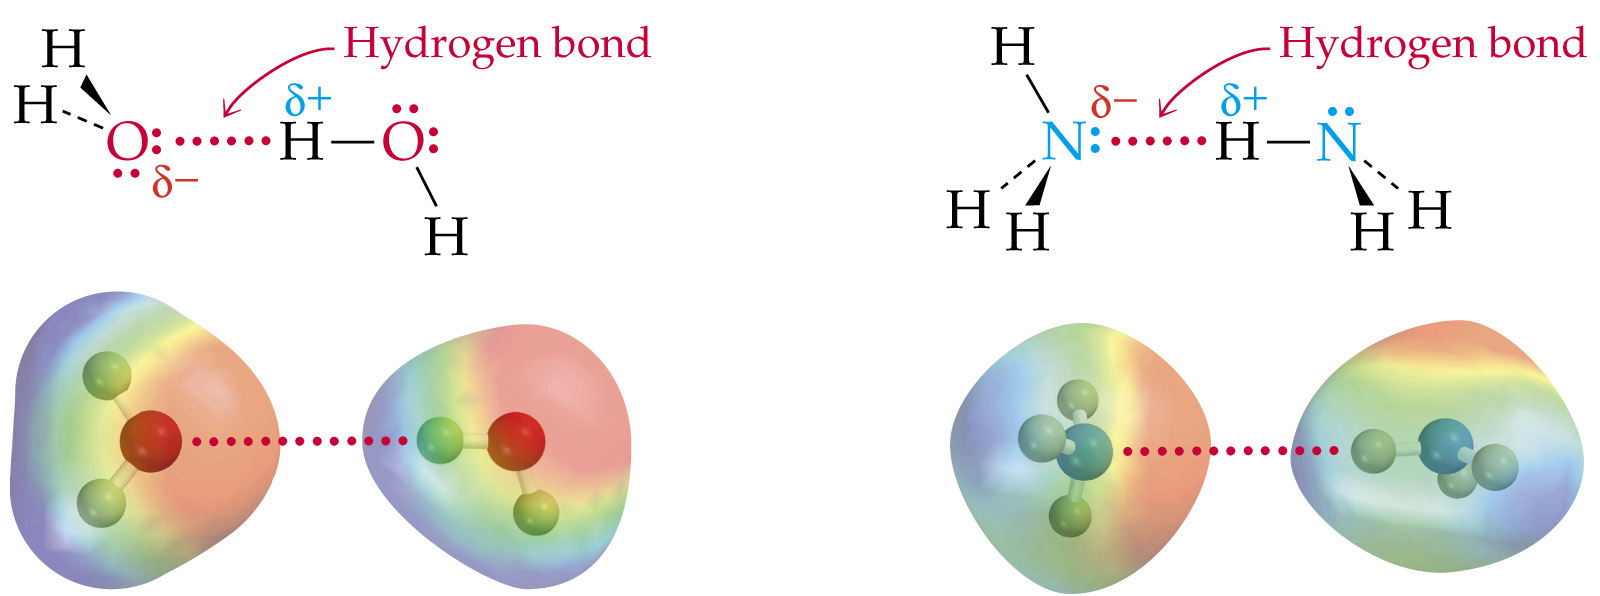
\includegraphics[width=\textwidth]{hydrogen}
\end{center}
\end{marginfigure}
\marginnote[2mm]{Hydrogen bonding with ammonia.}

\bigskip
An \emph{addition polymerization} begins with a molecule breaking down into two free radicals. A radical then attaches to a monomer molecule breaking the double bond, forming a new radical. This recursive procedure when the remaining original radical combines with the new polymer.

\bigskip
A \emph{condensation reaction} is one in which two monomers with functional groups combine to former a monomer and $H_2O$.

\section{Polymers}
A \emph{block copolymer} has repeated segments of each monomer, and a \emph{graft} copolymer has segments of one monomer branching off the main chain. Additionally, \emph{thermoplastic} polymers melt and deform upon heating, conversely of thermosetting ones.
%
\begin{marginfigure}[0mm]
\begin{center}
  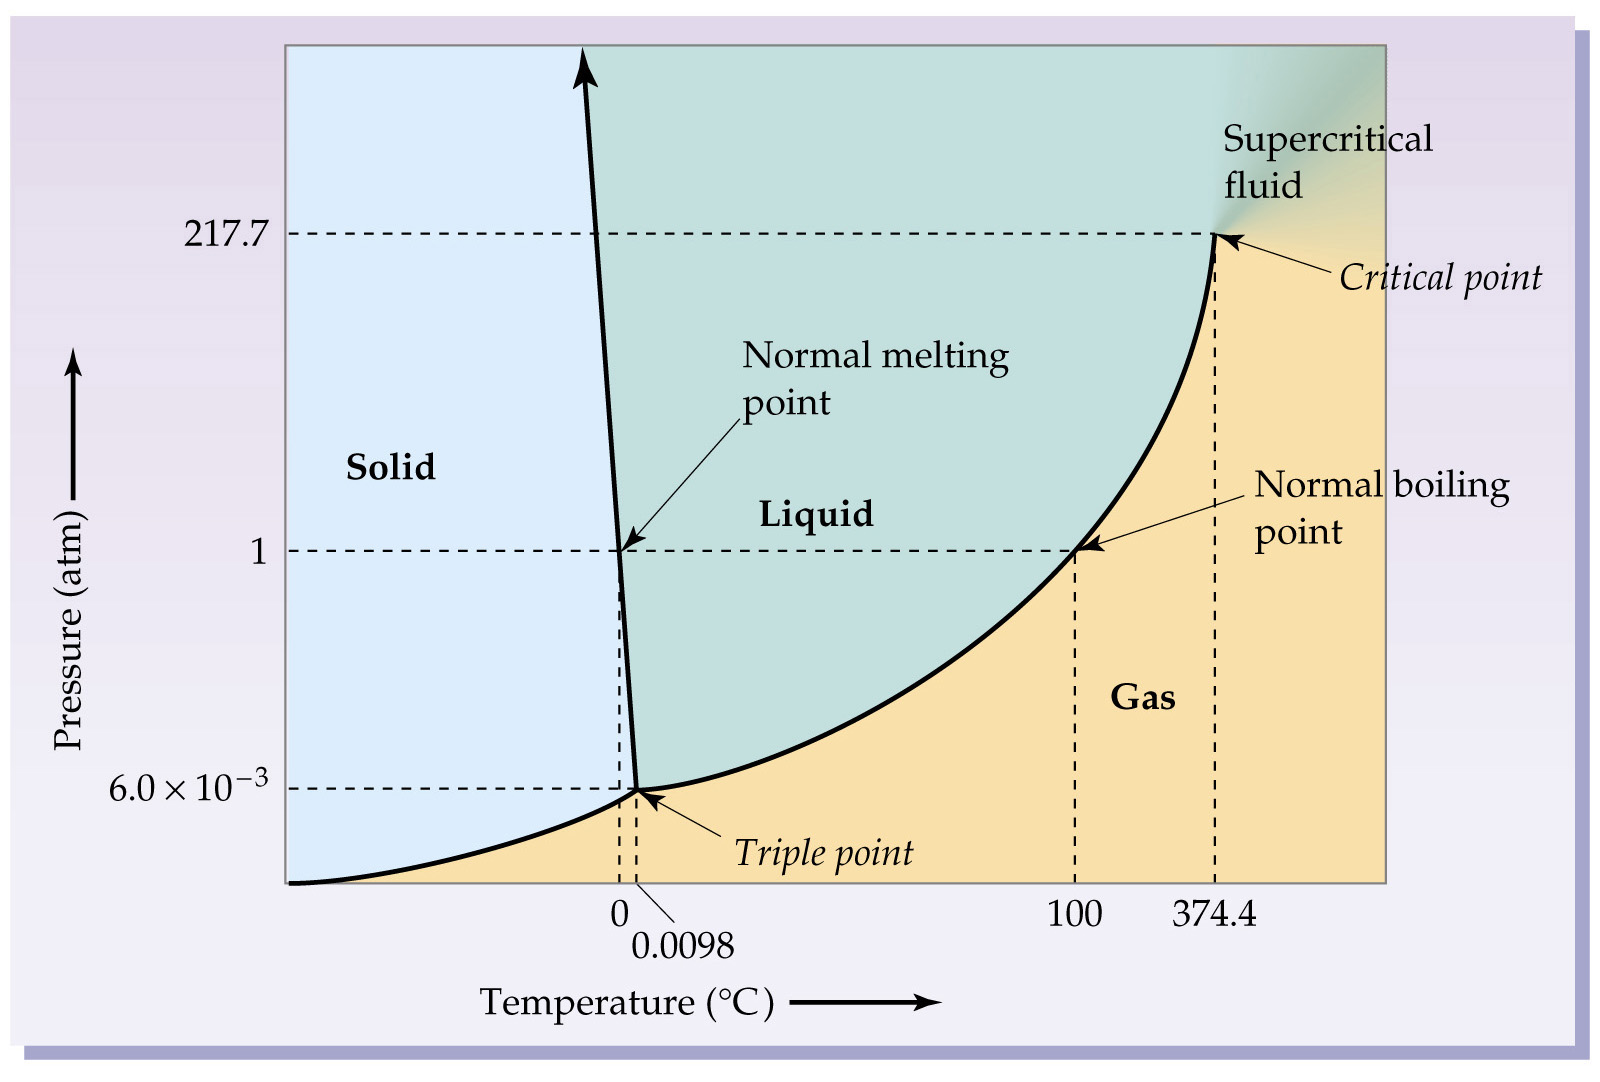
\includegraphics[width=\textwidth]{phases}
\end{center}
\end{marginfigure}
\marginnote[2mm]{The phase diagram of water.}

\bigskip
The \emph{degree of polymerization} is $\overline M / M_{mon}$ and the average molecular weight of such chains is
\begin{equation}
  \overline M_n = \frac{\sum MN}{\sum N} \quad\text{and}\quad \frac{\sum M^2 N}{\sum MN} \quad\text{for}\quad n_{\mathrm{chains}} = \frac{m N_a}{\overline M}
\end{equation}
The primary polymer structures are \emph{linear, branched, and crosslinked}. The former two are connected by non-bonded interactions and can be easily recycled, and the latter by covalent bonds. Linear polymers form crystal more easily and thus become liquid when heated.

% ------------------------------------------------------------------- %
% MISCELLANEOUS
% ------------------------------------------------------------------- %

\chapter{Miscellaneous}

\section{Organic Chemistry}

\textsc{Some common} functional groups include
%
\begin{center}
  \begin{tabular}{ll}
    Alcohol & --OH \\
    Ethers & --O-- \\
    Amines & --N-- \\
    Carboxylic & --C(=O)OH
  \end{tabular} \qquad\qquad
  \begin{tabular}{ll}
    Amides & --C(=O)N-- \\
    Aldehydes & --C(=O)H \\
    Ketones & --C(=O)-- \\
    Esters & --C(=O)O--
  \end{tabular}
\end{center}
%
LDPE and HDPE are linear and branched versions of polyethylene.
%
\begin{marginfigure}[0mm]
\begin{center}
  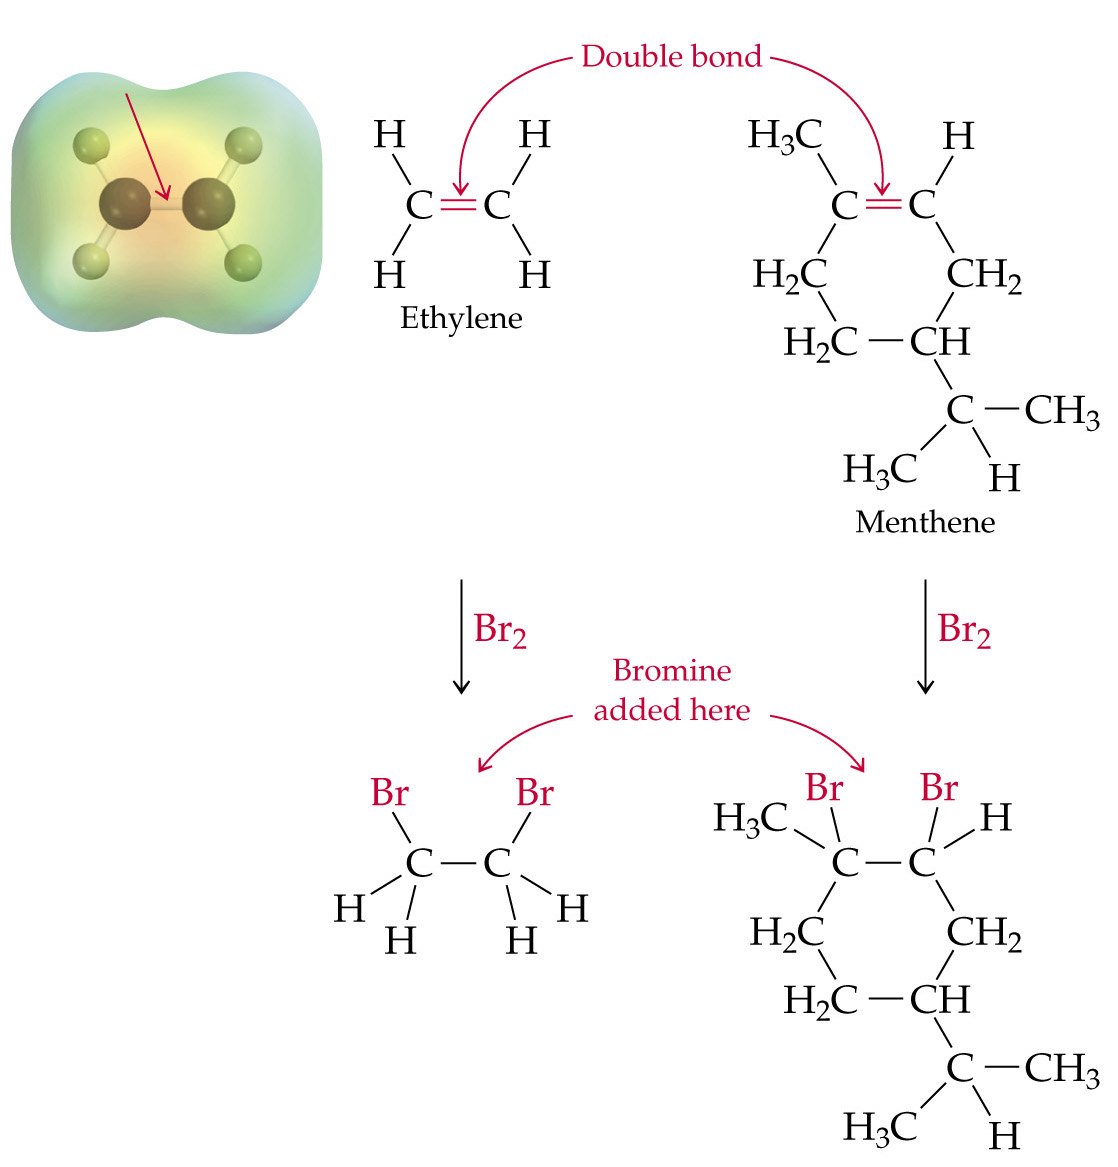
\includegraphics[width=\textwidth]{organic}
\end{center}
\end{marginfigure}
\marginnote[2mm]{Breaking a double bond when adding a molecule. Similar to an addition reaction.}

\section{Energetics}
The \emph{ionization energy} is the energy required for the reaction $A \to A^+ + e^-$. Conversely, \emph{electron affinity} is the energy required for $B + e^- \to B^-$.

\bigskip
The \emph{lattice energy} is defined as $U_{lat} = |\Delta H^\ominus_{lat}|$, and is proportional to $q$ and inversely proportional to $r$. This energy occurs in formation reactions $A^+ + B^- \to AB$ when $\Delta H_\ell < 0$.

\section{Gases}

The \emph{partial pressure} of one gas is
\begin{equation}
  P_i = X_i P \quad\text{for}\quad X_i = n_i/\sum n \quad\text{and}\quad P = \sum P_i
\end{equation}
Consequently, or a reactant $A$ dissociated $\delta \%$, then \begin{equation}
  P_A = (1- \delta)x \quad\text{and}\quad P_B = (v_B \delta / v_A)x
\end{equation}
where $x_i$ is the mole fraction, \begin{equation}
  x_i = \frac{m_i}{m} \frac{M}{M_i} = \frac{n_i}{n}
\end{equation}



\end{document}
